\subsection{Production deployment requirements}
\textit{This section explains what a production deployment is and what requirements it must met.}
~\\

\subsubsection{Multiple environments in software deployment}
First, it is helpful to distinguish between the terms: \textbf{'infrastructure stack' and 'environment'}. They both may be defined as a collection of infrastructure resources. The difference is that \textbf{an environment is conceptual, while a stack is concrete}. A stack is defined with code, particularly when Infrastructure as Code is applied, and managed using tools. However, an environment serves to fulfill a predetermined purpose. Multiple environments can run an instance of the same system\cite{book-iac}.

Typically, there are \textbf{two reasons for which multiple environments are in use}: to support a release delivery process and to run multiple production instances of the system. The first reason allows to have a particular build of an application (e.g. a git commit or a specified version of code) well tested. Such a build has to go through many different environments, e.g.: testing, staging and production. When a build does not pass all the stages in the former environments, it will not be promoted to the production environment\cite{book-iac}\cite{book-cicd}.

To briefly explain the second reason for multiple environments: they are used in order to ensure fault-tolerance (when one environment fails, the other can take over), scalability (the work can be spread among many clusters), segregation (it may be decided to handle a group of customers using one environment and the other group with the other environment, e.g. for latency purposes)\cite{book-iac}. Well-known examples of running multiple production deployments can be \textbf{Blue-green deployments or Canary deployments}\cite{bachelor-ha}.

\subsubsection{Production deployment requirements}
\label{Production deployment requirements}
Throughout this work a production deployment means such a deployment which targets the production environment. A list of \textbf{requirements for a production deployment}, gathered through the literature, is provided below:
\begin{itemize}
\item \textbf{Central Monitoring} - this is helpful when troubleshooting a cluster\cite{book-mastering-k8s}\cite{online-weave-checklists}\cite{online-weave-guide}\cite{book-cndwk}.
\item \textbf{Central Logging} - this is a fundamental requirement for any cluster with number of nodes or pods or containers greater than a couple\cite{book-mastering-k8s}\cite{online-weave-checklists}\cite{book-devops-k8s}.
\item \textbf{Audit} - to show who was responsible for what action\cite{online-weave-guide}.
\item \textbf{High Availability} - authors of \cite{book-mastering-k8s} go even further and state that the cluster should be tested for being reliable and highly available \textbf{before} it is deployed into production\cite{book-mastering-k8s}\cite{book-cndwk}.
\item \textbf{Live cluster upgrades} - it is not affordable for large Kubernetes clusters with many users to be offline for maintenance\\cite{book-mastering-k8s}.
\item \textbf{Backup, Distaster Recovery}\cite{book-mastering-k8s}\cite{online-weave-guide}\cite{book-cndwk}.
\item \textbf{Security, secrets management, image scanning} - security at many levels is needed (node, image, pod and container, etc.)\cite{book-mastering-k8s}\cite{online-weave-checklists}\cite{online-weave-guide}\cite{book-cndwk}.
\item \textbf{Passing tests, a healthy cluster} - 'if you don't test it, assume it doesn't work'\cite{book-mastering-k8s}\cite{book-cndwk}.
\item \textbf{Automation and Infrastructure as Code} - in production environment a versioned, auditable, and repeatable way to manage the infrastructure is needed\cite{book-mastering-k8s}\cite{online-weave-guide}.
\item \textbf{Autoscaling} - if application deployed on a Kubernetes demand more resources, then a new Kubernetes node should be automatically created and added to the cluster. However, autoscaling, even though nice to have, is not that important\cite{book-cndwk}.
\end{itemize}

\subsubsection{Monitoring as production environment requirements}
\textbf{Monitoring} helps to ensure that a cluster is operational, correctly configured and that there are enough resources deployed. Monitoring is also indispensable for debugging and troubleshooting\cite{book-mastering-k8s}. The third reason for using a monitoring system is that historical data is needed for planning purposes. The monitoring strategy should cover four areas\cite{book-cicd}:
\begin{itemize}
\item configuring the infrastructure in such a way that it is possible to collect the data,
\item storing the data,
\item providing dashboards, so that data is presented in a clear way,
\item setting up notifications or alarms to let people know about certain events.
\end{itemize}
\paragraph{}
Monitoring provides various \textbf{metrics}, e.g.: CPU usage, memory utilization, I/O per disk, disk space, number of network connections, response time, etc. Thus, it is helpful on many different levels: on hardware, operating system,  middleware and application level. There is a wide range of \textbf{available open source and commercial tools} to take care of monitoring: Nagios, OpenNMS, Flapjack, Zenoss, Tivoli from IBM, Operations Manager from HP, Splunk, etc.\cite{book-cicd}. Solutions recommended for a Kubernetes cluster are: Heapster combined with InfluxDB as backend and Grafana as frontend and also cAdvisor\cite{book-mastering-k8s}. A nice feature of Grafana are its dashboards. Example Grafana dashboard is presented in the next image:
\begin{figure}[H]
  \centering
  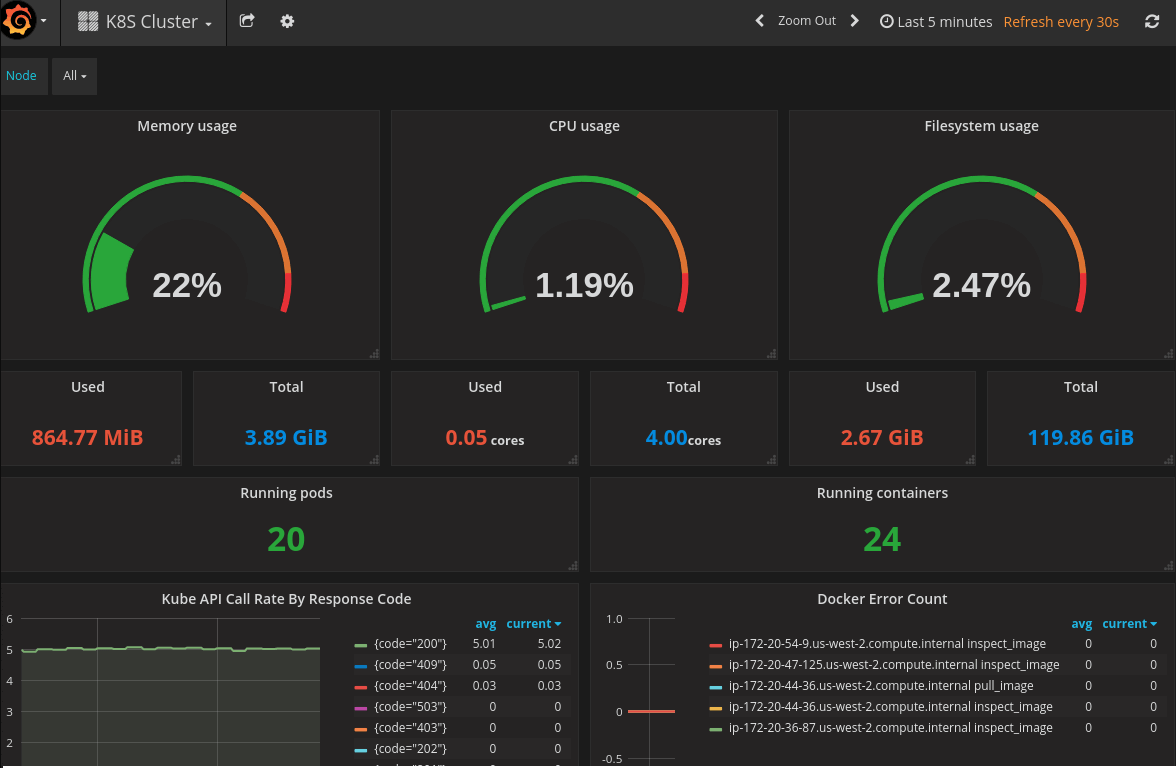
\includegraphics[width=11cm]{figures/grafana.png}
  \label{fig:grafana}
  \caption{Example Grafana dashboard for a Kubernetes cluster\cite{monitor-kubernetes-cluster-prometheus-grafana}}
\end{figure}
Grafana also works well with Prometheus, which is a monitoring system and a time series database. Prometheus is also a CNCF graduated project\cite{online-prometheus-gh}\cite{online-prometheus-www}. If a system (like Kubernetes) is deployed on AWS, another solution for monitoring and logging may be: Amazon CloudWatch\cite{online-cw}.

Another solution for monitoring is Kubernetes dashboard, which is a built-in solution and doesn't require any customization. Heapster, InfluxDB and Grafana are great for heavy-duty purposes, whereas Kubernetes dashboard is probably able to satisfy the majority of monitoring needs of a Kubernetes cluster\cite{book-mastering-k8s}\cite{book-devops-k8s}. Example dashboard provided by Kubernetes dashboard is depicted on the next image:
\begin{figure}[H]
  \centering
  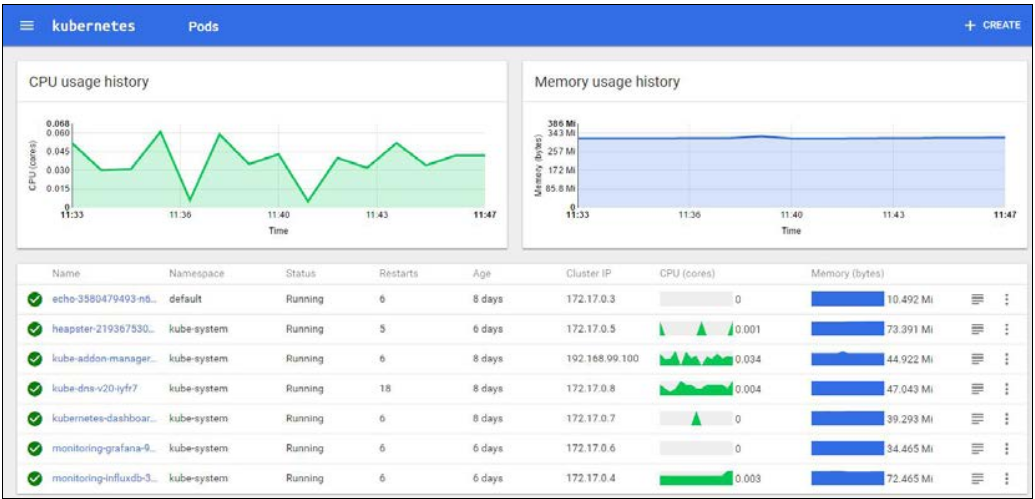
\includegraphics[width=10cm]{figures/k8s-dashboard.png}
  \label{fig:grafana}
  \caption{Kubernetes dashboard in action}
  \\
  \small{Source: \cite{book-mastering-k8s}, p. 53}
\end{figure}

\subsubsection{Logging as production environment requirements}
Kubernetes dashboard has also a feature which makes it able to show \textbf{log messages} of a single container deployed on Kubernetes\cite{book-mastering-k8s}. \textbf{Centralized logging} is essential for a production cluster, because usually there are a lot of pods (and containers) deployed, each generating many log messages. It is impossible to require a Kubernetes administrator to log into each container for the purpose of getting the logs. The second reason for the importance of centralized logging is that containers are ephemeral - the log messages kept inside the containers would be lost after a container is redeployed. \textbf{Popular solutions} are: Fluentd, Elasticsearch, Kibana\cite{book-mastering-k8s}, Logstash\cite{book-devops-k8s} and Graylog\cite{online-prod-year-k8s}\cite{online-graylog}. It is also important to consider that log messages in Kubernetes cluster are generated from many sources: from end-user applications, nodes, Kubernetes system containers and there are also \textbf{audit logs} in the form of e.g. api server events\cite{online-graylog-art}. For the purposes of auditing, when deploying on AWS, one can use AWS CloudTrail\cite{online-ct}.

\subsubsection{High Availability as production environment requirements}
While administering a Kubernetes cluster, there is a high probability that something will go wrong. Components, network can fail, configuration can be incorrect, people make mistakes and software has bugs. Failure classification has been described in \cite{article-failures}, p. 5. This has to be accepted and a system should be designed in such a way that it is \textbf{reliable and highly available (HA)} despite of many problems. Here is a list of ideas how to ensure high availability\cite{book-mastering-k8s}:
\begin{itemize}
\item \textbf{Redundancy} - means having a spare copy of something. Kubernetes uses Replica Sets or Replication Controllers to provide redundancy for applications deployed on Kubernetes. Five redundancy models were summarized in \cite{article-redundancy-models}, p. 978-980. Some of them require an active replica (running) and other passive (or standby).
\item \textbf{Hot Swapping} - can be explained as replacing some failed component on the fly, with minimal or ideally zero down-time. Actually, hot swapping is quite easy to implement for stateless applications. For stateful applications, one has to keep a replica of a component (see redundancy).
\item \textbf{Leader election} - it is a pattern used in distributed systems. Whenever there are many servers fulfilling the same purpose to share the load. One of the servers must be elected a leader then and certain operations must go through it. When the leader server experiences a failure, other server can be selected as new leader. This is a combination of redundancy and hot swapping.
\item \textbf{Smart load balancing} - used to share and distribute the load.
\item \textbf{Idempotency} - means that one request (or some operation) is handled exactly once.
\item \textbf{Self-healing} - means that whenever a failure of one component happens, it is automatically detected and steps are taken (also automatically) to get rid of the failure.
\item \textbf{Deploying in a cloud} - a goal is to be able to physically remove or replace a piece of hardware, either because of some issues or because of preventative maintenance or horizontal growth. Often this is too expensive or even impossible to achieve\cite{article-failures}. Traditional deployments on-premises forced administrators to do a capacity planning (to predict the amount of computing resources). Thanks to the on-demand and elastic nature of the clouds, the infrastructure can be closely aligned to the actual demand. It is also easy to scale applications deployed on a cloud, because of the fundamental property of the cloud: elasticity\cite{article-aws-architecting}.
\end{itemize}

Generally speaking, \textbf{"highly available systems are fault tolerant systems with no single point of failure"\cite{article-redundancy-models}. In order to introduce HA for the Kubernetes cluster the following ideas could be incorporated\cite{book-mastering-k8s}:
\begin{itemize}
\item Deploy Etcd as a cluster, not just one instance of Etcd.
\item Ensure redundancy for api server.
\item Deploy multiple master instances and ensure a load balancer in front of them.
\item Ensure that node instances are reliable: the Docker daemon and the Kubelet daemon should restart automatically in case of failure.
\item Apply RAID to ensure redundancy of data storage or apply Key-Value Multi-Device (KVMD), a hybrid data reliability manager\cite{data-rel-kv} or let cloud provide storage availability.
\end{itemize}

Furthermore, it may be needed to test high availability. This can be done by inducing a predictable failure and verifying if the system behaves as expected\cite{book-mastering-k8s}. Such a kind of testing, where one or more cluster nodes or pods is killed is called Chaos Monkey, after the tool developed by Netflix. There are also ready to use tools basing on the idea of Chaos Monkey: chaoskube, kube-monkey, PowerfulSeal \cite{book-cndwk}.
\begin{figure}[H]
    \centering
    
\includegraphics[width=5cm]{figures/chaos-monkey-logo.png}
    \label{fig:chaos-monkey-logo}
    \caption{Logo of the Netflix program: Chaos Monkey}
    \small{Source: https://netflix.github.io/chaosmonkey/, (accessed 17.04.2020)}
\end{figure}

\subsubsection{Automation as production environment requirements}
When it comes to \textbf{automation}, many guidelines can be found in \cite{book-cicd}, p. 13-29. Below are some of them listed:
\begin{itemize}
\item \textbf{Every Change Should Trigger the Feedback Process} - means that every change in code should trigger some pipeline and should be tested (including unit tests, functional acceptance tests, nonfunctional tests). The tests should happen in an environment which is as similar as possible to production. Some tests may run in production environment too\cite{book-cicd}\cite{book-iac}.
\item \textbf{The Feedback Must Be Received as Soon as Possible} - this also involves another rule: fail fast. This guideline suggests that faster tests (or less resource-intensive tests) should run first. If theses tests fail, the code does not get promoted to the next pipeline stages, which ensures optimal use of resources\cite{book-cicd}.
\item \textbf{Automate Almost Everything} - generally, the build process should be automated to such extent where specific human intervention or decision is needed. But there is no need to automate everything at once\cite{book-cicd}\cite{book-iac}.
\item \textbf{Keep Everything in Version Control} - this means that not only application source code but also tests, documentation, database configuration, deployment scripts, etc. should be kept in version control and that it should be possible to identify the relevant version. Furthermore, any person with access to the source code should be able to invoke a single command in order to build and deploy the application to any accessible environment. Apart from that, it should be also clear which version in version control was deployed into each environment\cite{book-cicd}.
\item \textbf{If It Hurts, Do It More Frequently, and Bring the Pain Forward} - if some part of the application lifecycle is painful, it should be done more often, certainly not left to do at the end of the project\cite{book-cicd}.
\item \textbf{Idempotency} - the tools used for automation should be idempotent, which means that no matter how many times the tool is invoked, the result should stay the same\cite{book-iac}.
\end{itemize}

\paragraph{}
Together with automation, there are two inextricably entwined terms: Infrastructure as Code and DevOps. As these two terms has been already explained in this work, now let us focus on the essential tools needed to introduce the automated application lifecycle. First, a framework for \textbf{Configuration Management} is needed. Examples involve: Puppet, CFEngine\cite{book-cicd}\cite{book-iac}, Chef\cite{online-chef}, Ansible\cite{online-ansible}, SaltStack\cite{online-salt}, etc. These tools help to declaratively define what packages should be installed and how should they be configured in a virtual machine or a container or a physical server\cite{book-cicd}. They can help prevent \textbf{configuration drift} in a large number of computers\cite{book-devops-k8s}. A configuration drift is a difference across systems that were once identical. It can be imposed by a manual amendment and also by automation tools which propagated a change only to some of the instances\cite{book-iac}. There are also stack-oriented tools, which follow the same declarative model: Terraform and CloudFormation\cite{book-iac}. Another type of needed tools is a building server, examples are: Jenkins, GoCD, Travis - they were already mentioned earlier.

\subsubsection{Security as production environment requirements}
\textbf{Security} is another essential aspect of production deployment and, as mentioned above, it touches many levels. A node breach is a very serious problem and it can happen by someone logging to the instance or having physical access to it. The latter is easily mitigated by not deploying on bare-metal machines but on a cloud instead\footnote{\cite{book-mastering-k8s}, p. 92, 93}. The former demands some hardening done. There are several ideas that can be implemented for a Kubernetes cluster specifically listed below:
\begin{itemize}
\item ensuring that data is encrypted in transit by using secure api server protocol (HTTPS instead of HTTP)\footnote{\cite{book-mastering-k8s}, p. 93, 113}.
\item ensuring proper user and permissions management by configuring authentication, authorization, security accounts and admission control in api server \footnote{\cite{book-mastering-k8s}, p. 93, 98, 104}. When setting up authorization, it is wise to apply \textbf{the principle of least privilege}. This principle recommends that only the needed resources or permissions should be granted\footnote{\cite{book-cndwk}, p. 141}.
\item utilizing Role-Based Access Control (RBAC) to manage access to a cluster\footnote{\cite{book-cndwk}, p. 199}.
\item ensuring security keys management and exchange\footnote{\cite{book-mastering-k8s}, p. 93} by implementing for example automated key rotation.
\item ensuring that used Docker images are neither malicious (deliberately causing some harm) nor vulnerable (allowing some attacker to take control) by keeping them up-to-date and maintaining them instead of using the publicly available ones or by using a private Docker registry\footnote{\cite{book-mastering-k8s}, p. 95, 96, 105}.
\item using minimal Docker images because the fewer programs there are installed in an image, the fewer potential vulnerabilities there are\footnote{\cite{book-cndwk}, p. 26}.
\item maintaining a log or audit system\footnote{\cite{book-mastering-k8s}, p. 98}.
\item utilizing network policies which act in a whitelist fashion and can open certain protocols and ports\footnote{\cite{book-mastering-k8s}, p. 113}.
\item using secrets. Kubernetes has a resource called: secret, but the problem is, that Kubernetes stores secrets as plaintext in Etcd. This, in turn, means that steps should be taken in order to limit direct access to Etcd\footnote{\cite{book-mastering-k8s}, p. 113}.
\item prefering managed services, because they will have many security measures already implemented\footnote{\cite{book-cndwk}, p. 41}.
\item avoid running processes as root user in Docker containers\footnote{\cite{book-cndwk}, p. 105, 142}.
\item using available programs for security scanning\footnote{\cite{book-cndwk}, p. 204}.
\end{itemize}

The following illustration presents security features available by api server:
\begin{figure}[H]
    \centering
    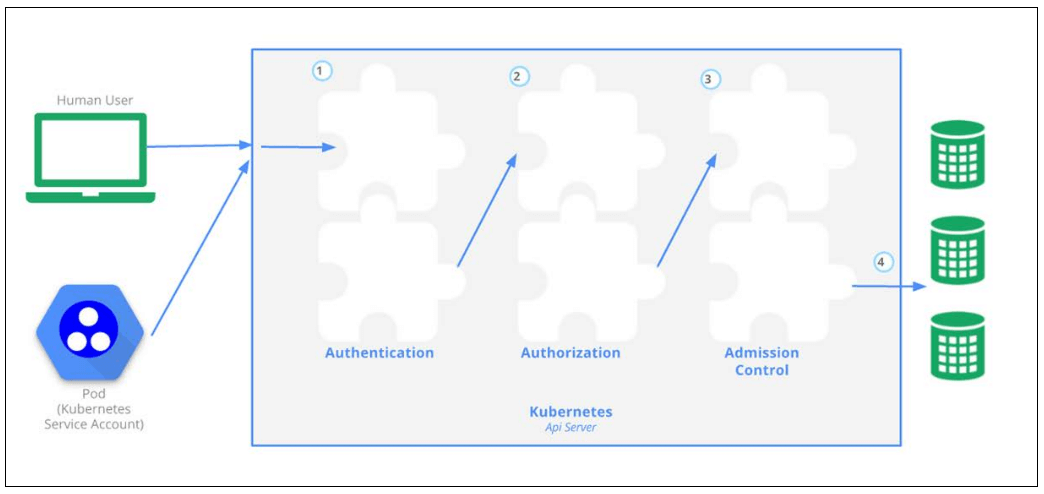
\includegraphics[width=13cm]{figures/security-api-server.png}
    \label{fig:security-api-server}
    \caption{An example test and release process diagram}
    \small{Source: \cite{book-mastering-k8s}, p. 101}
\end{figure}

There are many more security measures that Kubernetes administrators and end-users could apply. An interested reader is referred to\cite{book-cndwk}, p. 141-151, 199-205 and \cite{book-mastering-k8s} p. 91-119.

\textbf{Disaster recovery} can be understood as the process which an organization has to undergo after a service  disruption happened in order to resume normal services. It is vital to know what actions are necessary to overcome the disaster. This set of predefined procedures is known as \textbf{Disaster Recovery Plan}. Furthermore, disaster recovery is not the same as fault tolerance. The latter ensures that a system will withstand and resist the failure\footnote{\cite{article-dr}, p. 1, 2}.

Disaster recovery is an essential requirement of any business where continuity matters. In order to plan disaster recovery well the following key parameters should be considered: the initial cost, the cost of data transfers and the cost of data storage. Significant costs may be a reason why, in the past, around 40-50\% of small businesses had no DRP and did not intend to change this. However, cloud computing provides affordable solutions, because of the employed model "pay-for-what is used". Another advantage of the cloud is that it is fairly easy to use resources deployed in multiple geographical areas. This is desired, because one the major concepts in a DRP is the geographical separation of the system servers and its backup\footnote{\cite{article-dr-cloud}, p. 1, 2}.

Key metrics that can be taken into consideration while planning disaster recovery are\footnote{\cite{article-dr}, p. 2, \cite{article-dr-cloud}, p. 3}:
\begin{itemize}
\item Critical Business Function (CBF)
\item Maximum Acceptable Outage (MAO)
\item Recovery Point Objective (RPO)
\item Recovery Time Objective (RTO)
\item Business Impact Analysis (BIA)
\end{itemize}
RPO can be defined as the time between two successive backups. Thus, the time between the last backup and the the disaster, which is de facto the time of data loss, is maximally equal to RPO. RTO can be understood as the time needed to recover from the disaster, when the server experiences downtime\footnote{\cite{article-dr-cloud}, p. 3}. RPO and RTO are illustrated on the following image:
\begin{figure}[H]
    \centering
    
\includegraphics[width=13cm]{figures/rpo-rto.png}
    \label{fig:rpo-rto}
    \caption{RPO and RTO}
    \small{Source: Own work}
\end{figure}

Cloud services mitigate some risks that persistent data storage has. For example: cloud services provide high-available data storage by replicating it across different geographical locations. However, replication is not the same as backup and it does not protect against accidentally deleting a volume or against a misconfigured application overwriting the data. Thus, backup is still needed. In order to backup Kubernetes, the Etcd database has to be backuped. Apart from that, each application deployed on top of Kubernetes should be backuped on its own\footnote{\cite{book-cndwk}, p. 206, 207}. There are already available services that help with Kubernetes backup: Velero\footnote{\cite{book-cndwk}, p. 208-211}.

The last thing that is explained in this section is \textbf{testing}. Before the production Kubernetes cluster is ready for end-users, it must be verified that it is healthy. Every component should be tested proving that it is working as expected, every node should be able to connect to a Docker registry, etc. Sometimes, applications, including the Kubernetes component: kube-scheduler, expose a custom \textbf{health endpoint}\footnote{\cite{book-devops-k8s}, p. 579, 580, 717}. Thanks to that, it is possible to verify regularly that a service is performing correctly. The solution is to send a request to the health endpoint. Usually, a HTTP response code of 200 indicates correct status of the service\footnote{\cite{online-ms-health}}. Kubernetes can monitor the health endpoints with \textbf{liveness probes}. Based on a specified health endpoint response, Kubernetes can restart the faulty container\footnote{\cite{online-k8s-probes}}.

The tests should be incorporated into a CICD pipeline. "Having a comprehensive test suite is essential to continuous integration" and test-driven development is a vital practice in this context\footnote{\cite{book-cicd}, p. 71}. There is even a possibility to implement \textbf{test-driven} changes to deployment environments. The recipe for achieving that is\footnote{\cite{book-cicd}, p. 292}:
\begin{enumerate}
\item Write such a check in a monitoring system that monitors the problem. Verify that the check is now failing.
\item Implement the change in configuration to the cluster.
\item Verify that, after the change is deployed, the monitoring check is passing.
\end{enumerate}
